\section{Results} \label{results}

\subsection{A new efficient \texttt{python} package}
Several algorithms to extract features from univariate time series had already been implemented in the \py{} package \pyeeg{}\citationneeded{}.
Unfortunately, some of them were critically slow, and could therefore not realistically have been used in the present study.
Preliminary investigation of \pyeeg{} source code revealed that runtimes may be improved by vectorising expressions and pre-allocating of temporary arrays.
Therefore, systematic reimplementation of all algorithms in \pyeeg{} was undertaken.
Very significant improvement in performance were achieved for almost all functions(table~\ref{tab:benchmark}).
Critically, sample \citationneeded{} and absolute \citationneeded{} became usable in reasonable time.
\begin {table}[!h]
\begin{center}
\caption{\ctit{Performance improvements over \texttt{PyEEG}.}
In order to improve performance, modifications of the algorithms implemented in \texttt{PyEEG} were carried out.
This table compares how long, on average, each algorithm would take, for a random sequence of length $1280$ (\ie{} $5s$ at $256$Hz).
It also represents how many added points would lead to a tenfold runtime increase.
For the tested range ($n \in [1280;7680] $), all algorithms add approximately an
exponential time complexity ($10^{O(n)}$, $R^2 > 0.95$, for all).
Several mathematical inconsistencies were also discovered and corrected. 
The rightmost column (\textbf{\textdagger}) indicates whether the original implementation was
corrected in order to match mathematical definition. Each alteration is mathematically justified in the section \texttt{pyrem.univariate} of the \pr{} documentation (see appendix).
\textbf{(-)}: indicates a worse performance of \pr{} over \pyeeg{}.
Significance levels: $^{***}$, $p-value < 10^{-3}$; $^{**}$, $p-value < 10^{-2}$, see Material and Methods for detail about statistical analysis.
\label{tab:benchmark}
}
\footnotesize
\begin{tabular}{|c|c|c|c|c|c|c|}
  \hline
  &  & \multicolumn{2}{|c|}{\texttt{PyEEG}} & \multicolumn{2}{|c|}{\pr} & \\
 \hline
 \hline
 
  algorithm & function & \specialcell{$t$(ms) for \\$n = 1280$} & \specialcell{$n$ for $\times 10$\\increase} & \specialcell{$t$(ms) for \\$n = 1280$} & \specialcell{$n$ for $\times 10$\\ increase} & fix\textsuperscript{\textdagger}\\
 
  \hline
  \hline
\specialcell{Approximate\\Entropy} & \texttt{ap\_ent} &                                     9970 & 4288 & $487^{***}$ & $3478^{***}(-)$ & No\\
\hline
Fisher Information & \texttt{fisher\_info} &                                 3.24 & 8673 & $0.121^{***}$ & $12427^{***}$ & No\\
\hline
\specialcell{Higuchi\\Fractal Dimension} & \texttt{hfd} &                     11.7 & 8833 & $1.39^{***}$ & $28329^{***}$ & Yes\\
\hline
Hjorth parameters & \texttt{hjorth} &                                         5.14 & 8633 & $0.088^{***}$ & $36354^{***}$ & Yes\\
\hline
\specialcell{Petrosian\\Fractal Dimension} & \texttt{pfd} &                 2.66 & 8606 & 2.65 & 8579 & Yes\\
\hline
Sample Entropy & \texttt{samp\_ent} &                                         8305 & 4276 & $188^{***}$ & $5483^{***}(-)$ & No\\
\hline
Spectral Entropy & \texttt{spectral\_entropy} &                                 0.309 & 11459 & $0.227^{***}$ & $22133^{***}$ & Yes\\
\hline
\specialcell[l]{Singular Value \\Decomposition\\ entropy} & \texttt{svd\_ent} &     3.25 & 8663 & $0.113^{***}$ & $11774^{**}$ & Yes\\
 \hline
\end{tabular}
\end{center}
\end{table}


Importantly, several mathematical inconsistencies between the original code and the mathematical definitions were also noticed.
This affected five of the eight reimplemented functions(table~\ref{tab:benchmark}).
Detail of the corrections performed are provided, as notes, in the documentation of the new package (see appendix).
Numerical results for the three other functions were consistent throughout optimisation.

In order to facilitate feature extraction, several data structures and routines were also implemented
in a new python package named \pr{}.
Briefly, extensions of \texttt{numpy} arrays providing meta-data, sampling frequency, and other attributes were used to represent time series.
User friendly indexing with string representing time was also developed.
In addition, a container for time series of discrete annotation levels, each linked to a confidence level, was built.
Importantly, a container for multiple time series, which supports heterogeneous (between time series) sampling frequencies was implemented.
The new package also provides visualisation, input/output, and wrappers for resampling and discrete wavelet decomposition.
Finally, unittests were implemented to ensure persistence of mathematical and programmatic validity throughout developmental stage.
A complete documentation of \pr{} is provided in the appendix of the report herein.
%%%%%%%%%%%%%%%%%%%%%%%%%%%%%%%%%%%%%%%%%%%%%%%%%%%%%%%%%%%%%%%%%%%%%%%%%%%%%%%%%%%%%%%%%%%%%%%%%%%%%%%%%%%%%%%%%%%%%%%%%%%

\subsection{Twenty variables can generate accurate predictions}
Including temporal information (see next section) results in multiplication the number of variable, rendering computation difficult, and prediction potentially less accurate.
Therefore, iterative elimination of variables based on their importance was undertaken.
Starting with all 164 variables, random forests were trained, and the number of features was reduced by a factor $1.3$  by eliminating the least important variables.
For each iteration, the stratified cross-validation error (see material and methods) was computed (fig.~\ref{fig:variable_elimination}).

\begin{figure}[h!]
  \centering    
    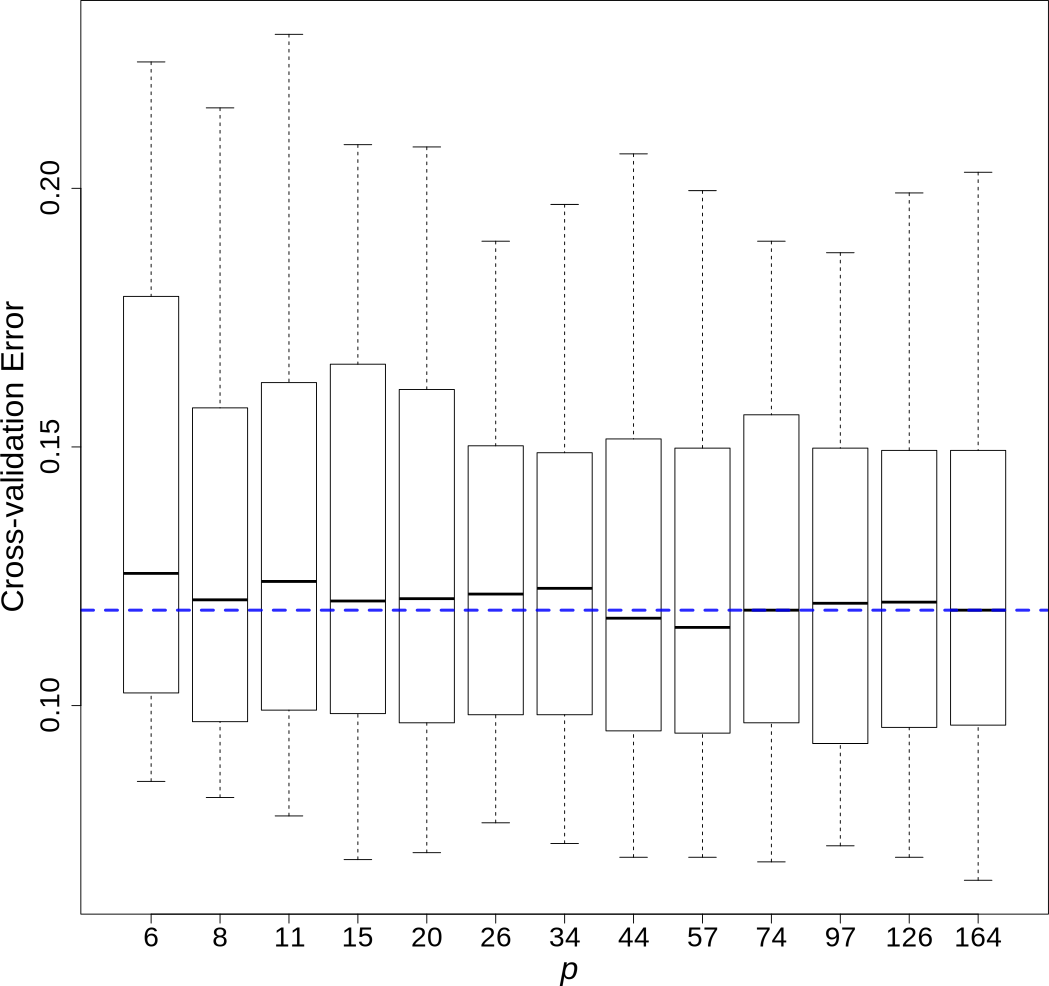
\includegraphics[width=0.5\textwidth]{figures/variable_elimination.pdf}
  \caption{\ctit{Recursive variable elimination.}
  Random forest were fitted recursively and only the most important $p/1.5$ variables were kept.
  Stratified cross-validation (see Material and Methods) was computed at each iteration. This procedure was replicated five time.
  The dashed blue line indicates the median cross-validation error when all variable are used.
  \label{fig:variable_elimination}
  }
\end{figure}

The predictive accuracy globally increases with the number of variables.
However, this increase is very moderate for ($p>8$) this indicates that dimensionality can be reduced without largely impacting accuracy.
For further investigation, $p=20$ was considered to be a good compromise between error and computational load.
\begin {table}[!h]
\begin{center}
\caption{\ctit{Relative variable importance of the 20 selected features.}
After recursive variable elimination, the 20 most important remaining features were used.

\label{tab:importances}}

\small
\begin{tabular}{|c|c|}
  \hline
  Feature family & features\\
 \hline
 \hline
  Power & \specialcell{\texttt{mean}, \texttt{sd}, \texttt{skewness}, \texttt{kurtosis}\\\texttt{median}, \texttt{min}, \texttt{max}}\\
  \hline
  Hjorth & \texttt{morbidity}, \texttt{complexity}\\
  \hline
  Fractal & \texttt{Petrosian} and \texttt{Higuchi} fractal dimensions\\
  \hline
  Entropy & \specialcell{\texttt{Fisher information}, \texttt{SVD entropy}\\and \texttt{Sample entropy} with $m=2$, and $ r \in \{ 0.2, 1.0, 1.5\}$}\\
 \hline


\end{tabular}
\end{center}
\end{table}


%%%%%%%%%%%%%%%%%%%%%%%%%%%%%%%%%%%%%%%%%%%%%%%%%%%%%%%%%%%%%%%%%%%%%%%%%%%%%%%%%%%%%%%%%%%%%%%%%%%%%%%%%%%%%%%%%%%%%%%%%%%

\subsection{Including temporal information improves prediction}
Manual scorer usually use contextual information in order to make a decision concerning a given state.
For instance, implicit assumptions are made on the temporal consistency of the states.
Therefore, it seems important to account for contextual information when building a predictor.
In this study, two different approaches were pursued.
Either the local means of features over different ranges were added to the features
of each epochs (eq.~\ref{eq:window}),
or the features of neighbouring time points were included (eq.~\ref{eq:tau}).

A comparison of both approaches is proposed in figure \ref{fig:temporal_integration}.
Significant improvement was achieved by both methods by including even little temporal information ($\tau = 1$, $n=\{1,3\}$).
The best accuracy was achieved with $\tau = 2$.
This value is also a good compromise in so far as it only inflates $p$ by five fold.
In addition, it is advantageous to require only five contiguous neighbouring epochs instead of having to integrate minutes of contextual information.
Combining both approaches did not improve prediction any further (data not shown).

\begin{figure}[h!]
  \centering    
    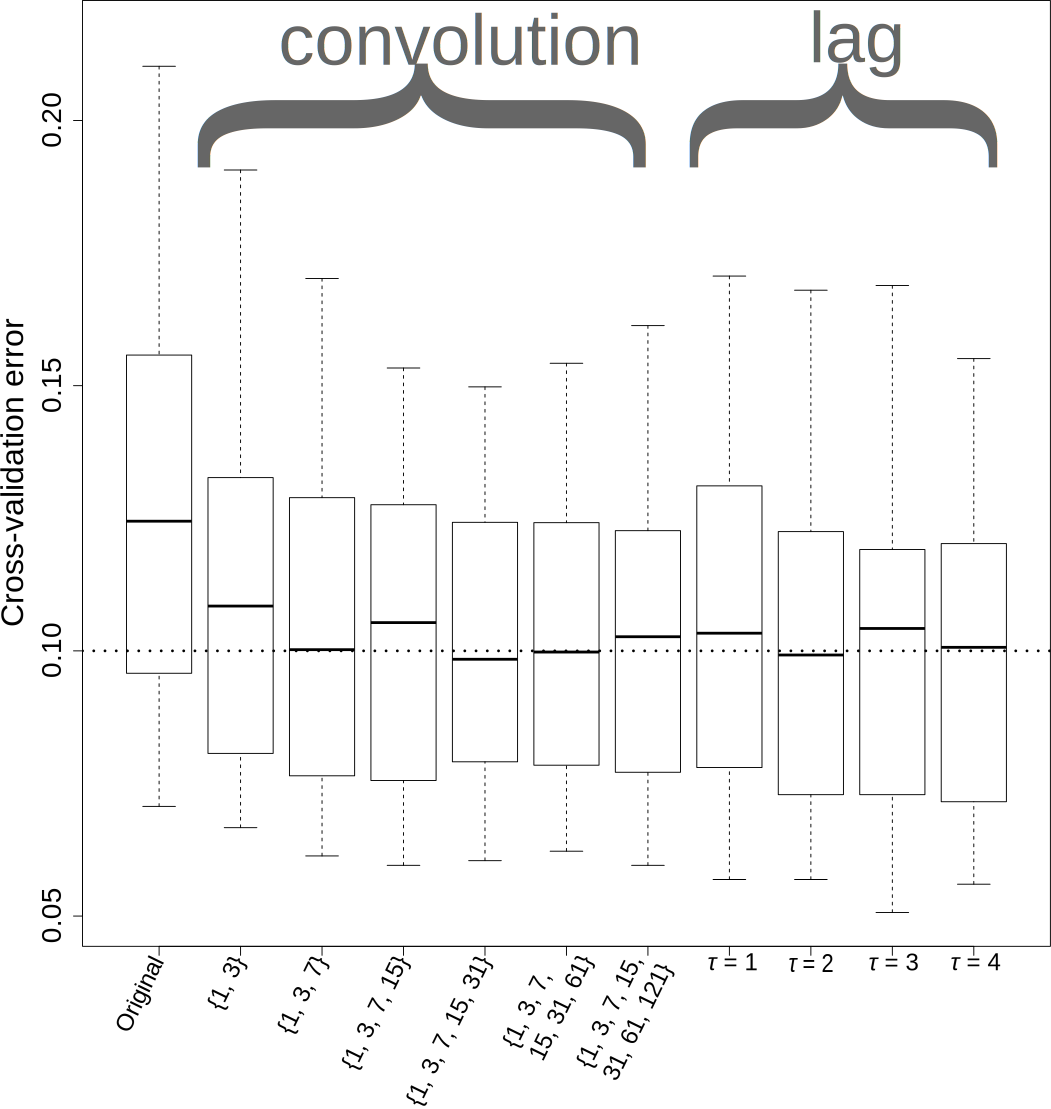
\includegraphics[width=0.5\textwidth]{figures/temporal_integration.pdf}
  \caption{\ctit{Integration of temporal information.}
  In order to improve prediction accuracy, information about the past and future features was added to the original features following two different strategies.
  Convolution inflates $p$ by adding the mean features of neighbouring points over different window sizes (eq.~\ref{eq:window}).
  The numbers in braces represent the window sizes.
  Alternatively, the features of the $\tau$ previous and future neighbours was added to the variables (eq.~\ref{eq:tau}).
  The dotted line represents a cross-validation error of $10\%$.
  All additions of temporal features reduce significantly the cross-validation error compared to the original set of features ($p-value < 5.10^{-3}$, for all, repeated t-tests).
  Significance threshold, $\alpha = 0.05$, after Bonferroni correction is $\alpha' = 0.05/10 = 5.10^{-3}$.
  \label{fig:temporal_integration}
  }
\end{figure}



\subsection{Structural differences with ground truth}

\begin{figure}[h!]
  \centering   
    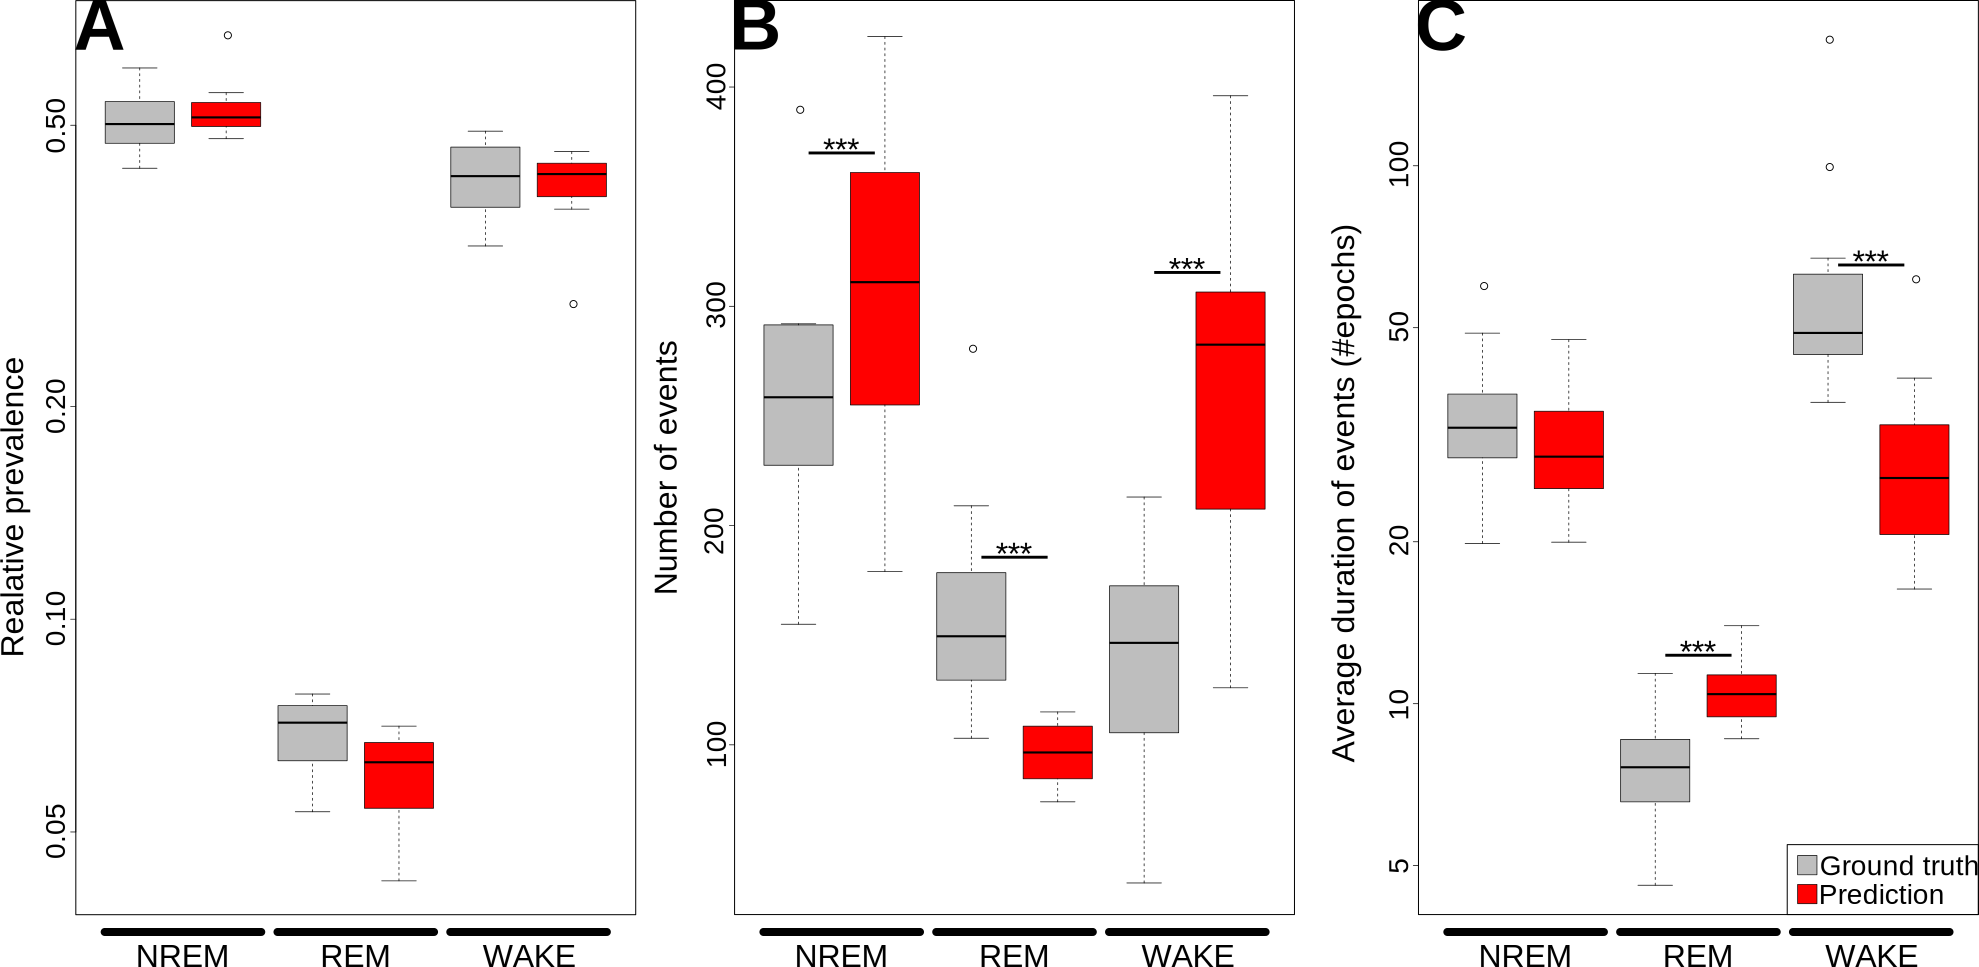
\includegraphics[width=1.0\textwidth]{figures/struct_assess.pdf}
  \caption{\ctit{Structural differences.}
  Three metrics describing structure of sleep were computed for both ground truth (grey) and predicted (red) time series.
  \textbf{A}, No significant difference in state prevalence was found.
  \textbf{B}, The number of events was significantly over-estimated by the classifier
   for wake state and under-estimated for \gls{rem} state ($p-value < 10^{-15}$ for both).
  \textbf{C}, The average duration of wake and \gls{rem} episodes
  were under-estimated ($p-value < 10^{-2}$) and marginally over-estimated ($p-value = 0.057$), respectively.
  Log scale was used for the response variables in A and C. 
  $n = 12$ per combination of factors.
  Statistical methods are detailed in the Material and Methods section.
  Significance levels: $^{***}$, $p-value < 10^{-3}$;  $^{**}$, $p-value < 10^{-2}$.
  \label{fig:struct_assess}
  }
\end{figure}


After selecting important variables and defining new ones, general and structural performance of the classifier was assessed.
For this purpose, random forests were trained on samples accounting for the unbalanced prevalence.
Predictions were generated using the same stratified sampling approach.
That is, predictions on each time series were made by a classifier for which
the training set did not contain any point from this time series.




\begin {table}[!h]
\begin{center}
\caption{\ctit{Relative confusion matrix.}
Agreement between reference scoring (rows) and proposed classifier (column).
For clarity, only the percentage of all epochs is shown.  The total number of epochs was 202171.
$a$, PPV (Positive Predictive Value = 1 - False Detection Rate); $b$, Overall Accuracy.
\label{tab:confus}
}
\footnotesize
\begin{tabular}{|c|c|c|c|c||c|}
  \hline
  & &   \multicolumn{3}{|c|}{Prediction} & \multirow{2}{*}{PPV$^a$} \\ 
  & & NREM& REM& WAKE &\\
  \hline
 \multirow{3}{*}{\specialcell{Ground\\truth}}
 
   & NREM & 47.9& 1.36& 3.03 & 0.92\\
   & REM & 0.63 & 5.14& 0.25 & 0.85\\
   & WAKE & 2.24& 0.42& 39.3 & 0.94\\
   \hline\hline
   \multicolumn{2}{|c|}{Sensitivity} &  0.94  & 0.74 &   0.92 &$0.92^b$\\
 \hline

\end{tabular}
\end{center}
\end{table}


The global confusion matrix is presented in table \ref{tab:confus}. The overall accuracy is 0.92.
For \gls{nrem} and wake, both specificity and positive predictive value were above 0.90. However
for \gls{rem} epochs, the specificity is only 0.74, and the false detection rate is 15\%.

In order to investigate the structural differences between ground truth and the predicted states,
three metrics describing physiological properties of sleep were computed (fig.~\ref{fig:struct_assess}).

Prevalence(fig.~\ref{fig:struct_assess}A) of states appears to be the most widely used metric to describe sleep patterns\citationneeded{}.
No significant difference was found between the ground truth and predicted prevalences ($p-value > 0.13$ for all, z test on the interaction terms of $\beta$ regression).

Sleep fragmentation is often assessed by a combination of two variables: number of episodes of a given state (fig.~\ref{fig:struct_assess}B) and average duration of all episodes per state (fig.~\ref{fig:struct_assess}C) \citationneeded{}.

Large differences were observed between the number of events computed from the ground truth or the predicted data.
($p-value < 10^{-15}$ for all, t test on the interaction terms of Poison GLMM).

Finally, significant differences were found between methods for the average durations of \gls{rem} ($p-value < 10^{-4}$) an wake ($p-value < 10^{-3}$) episodes
(t test on the interaction terms of linear mixed model).

\subsection{Attribution of confidence score to predictions}
Since classification can be inaccurate, it would be interesting to associate `confidence' score to each prediction.
A entropy based confidence metric $c$ (eq. \ref{eq:entropy}) was defined for this purpose.
In order to validate it, the average cross-validation error was computed for different degrees of confidence (fig\ref{fig:error}A).

\begin{figure}[h!]
  \centering    
	\includegraphics[width=1.0\textwidth]{figures/error.pdf}
	\caption{\ctit{A posteriori confidence assessement.}
	\textbf{A}, Relation between the confidence value derived from proportions of votes (eq.\ref{eq:entropy}) and actual proportion of error.
	Cross-validation accuracy increases with empirical confidence value.
	For low values of confidence, $[0, 0.1]$, the predictor is not very reliable (more that $45\%$ error, while random errors would be $67\%$).
	In contrast, within the highest confidence range, $(0.9, 1.0]$, miscalssifications are very rare($0.5 \%$).
	\textbf{B}, Distribution of confidence values for all epochs. The overall median confidence value is at 0.69.
	\textbf{C}, Visualisation of approximatly 30 minutes of representative recording. 
	The doubt level ($1 - c$) can be displayed on top of the prediction annotations.
	In this example, the ground truth is also displayed to demonstrate examples of missclassification.
	\label{fig:error}
  }
\end{figure}


As expected, the probability of misclassification decreases monotonically with $c$.
In addition, error rate seem to tend to zero when the confidence value is one, and, for confidences close to zero, the predictor is very inaccurate.
These characteristics indicate that $c$ can be used to as a supporting value for predictions.
One application of such a confidence level could be to provide user with an overall quality assessment.
In addition, it  makes it possible possible for the used to display while visually inspecting a recording (fig\ref{fig:error}C).
